\documentclass[12pt]{fphw}
%\usepackage{mathpazo}
%\usepackage[utf8]{inputenc}
%\usepackage[T1]{fontenc}
\usepackage{sectsty}
\usepackage{graphicx}
\usepackage{booktabs}
\usepackage{listings}
\usepackage{enumerate}
\usepackage{xcolor}

\sectionfont{\bfseries\large\raggedright}

\definecolor{codegreen}{rgb}{0,0.6,0}
\definecolor{codegray}{rgb}{0.5,0.5,0.5}
\definecolor{codepurple}{rgb}{0.58,0,0.82}
\definecolor{backcolour}{rgb}{0.95,0.95,0.92}

\title{Experiment 2}
\author{Aditya Kumar (24MAI14003)\\}
\date{08 Aug, 2024}
\institute{Chandigarh University\\Master of Engineeing---Artificial Intelligence}
\class{Artificial Intelligence Lab (24CSH-621)\\}
\professor{Dr. Manjit Singh}

\begin{document}

\maketitle

\section*{}
\begin{problem}
  \textbf{Aim: }Implement Informed (heuristic) search strategy for optimal shortest path and traffic navigational system. 
\end{problem}
\section{Theory}
The A* (A-Star) algorithm is a popular and highly efficient pathfinding and graph traversal 
algorithm often used in computer science, particularly for solving problems related to navigating 
through graphs or grids. It finds the shortest path between two nodes by considering both the actual 
cost from the start node to the current node (known as "g" cost) and an estimated total cost to 
reach the destination from the current node (known as "h" cost).
\section{Algorithm}
\begin{enumerate}
  \item Initialization: Create two lists - open list and closed list. The open list contains nodes that 
    need exploring, while the closed list contains nodes that have already been visited or evaluated. 
    Add the start node to the open list with a cost value equal to its "g" (actual) cost from the 
    starting position. 
  \item Loop until the open list is empty: 
    \begin{itemize}
      \item Find the node in the open list with the lowest f-cost, where `f(n) = g(n) + h(n)`, and break 
        the loop if it's a destination node (i.e., its position matches the goal).
      \item Move the selected node from the open list to the closed list.
    \end{itemize}
  \item Generate neighboring nodes: For each neighbor of the current node, calculate their "g" cost by 
    adding up the "g" value of the current node and the edge weight (distance) between them. Also, 
    estimate the "h" cost using a heuristic function such as Euclidean distance or Manhattan distance. 
  \item Check each neighboring node: 
    \begin{itemize}
      \item If the neighbor is not in the open list yet, add it there with its calculated values of g-cost 
        and h-cost (f-cost), along with a reference to the current node ("parent"). 
      \item If the neighbor already exists in the open list but has a higher g-cost than currently found 
        one, update its "g" cost value and set the current node as its new parent. This ensures that we're 
        always on the best path towards our goal. 
    \end{itemize}
  \item Repeat until you reach the destination: Keep repeating steps 2 to 4 until the open list is empty 
    or when a final destination has been reached. The algorithm will then return the shortest-path 
    sequence as a stack (or list) of nodes, where removing an element from the end of this structure 
    results in returning the optimal path.

\end{enumerate}
\section{Pseudocode}
    \begin{lstlisting}[language=Python, tabsize=2]
function reconstruct_path(cameFrom, current)
    total_path := {current}
    while current in cameFrom.Keys:
        current := cameFrom[current]
        total_path.prepend(current)
    return total_path
function A_Star(start, goal, h)
    openSet := {start}
    cameFrom := an empty map
    gScore := map with default value of Infinity
    gScore[start] := 0
    fScore := map with default value of Infinity
    fScore[start] := h(start)
    while openSet is not empty
        current := the node in openSet having the lowest fScore[] value
        if current = goal
            return reconstruct_path(cameFrom, current)
        openSet.Remove(current)
        for each neighbor of current
            tentative_gScore := gScore[current] + d(current, neighbor)
            if tentative_gScore < gScore[neighbor]
                cameFrom[neighbor] := current
                gScore[neighbor] := tentative_gScore
                fScore[neighbor] := tentative_gScore + h(neighbor)
                if neighbor not in openSet
                    openSet.add(neighbor)
    return failure
    \end{lstlisting}
\section{Code}
    \lstinputlisting[language=Python, backgroundcolor=\color{backcolour}, numbers=left, tabsize=2,basicstyle=\ttfamily\footnotesize, breaklines=true]{e2.py}
\section{Output}
    \begin{center}
      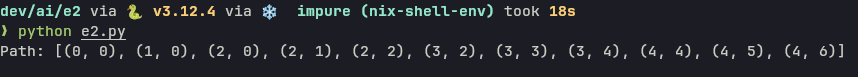
\includegraphics[width=0.6\columnwidth]{./e2.png}
    \end{center}
\section{Learning Outcomes}
\begin{enumerate}
  \item Understanding of graph theory 
  \item Implementation of informed search strategy 
  \item Search strategy evaluation
\end{enumerate}
\end{document}
